\chapter{Introduction} \label{introduction}

DNA sequencing allows us to read an organism's genome and, through software, 
learn more about its inherent capabilities without having to study it \textit{in 
vivo} or \textit{in vitro} \cite{de2012bioinformatic}. In an environmental 
microbiology context, such sequenced genomes are used to learn more about 
microorganisms' metabolic capabilities and possibly shed light on their 
ecological role \cite{de2012bioinformatic}. In an applied context, predictions 
of such metabolic capabilities are also useful for the selection of what 
microbes to use in a bioprocess. In a genetic engineering context, genomically 
derived information can be used to select what metabolic traits to remove from, 
or move between, organisms \cite{strohl2001biochemical,sanchez2005novel}.

Advances in DNA sequencing technology over the past decade have revolutionized 
our ability to acquire bacterial and archaeal genomes. For example, with newer 
sequencing technologies, such as Oxford Nanopore \cite{jain2016oxford}, a 
bacterial genome can be acquired in a matter of hours \cite{Lu2016,Cao2017}. 
Researchers have now moved on to extracting the genomes of unculturable 
microorganisms from environmental samples using culture-free techniques, such as 
metagenomic \cite{quince2017shotgun} and single-cell \cite{gawad2016single} 
sequencing. Over the past few years, the tree of life has been significantly 
expanded by the \gls{mags} \cite{bowers2017minimum} of these unculturable 
organisms \cite{Hug2016,Parks2017}. With microbiologists' inability to gather 
new genomes rectified, the problem now shifts to interpreting this new wealth of 
genomic data.

Due to their vast size and information density, the interpretation of genomes is 
often assisted by software. The tool developed as part of the thesis work, 
Micromeda, allows users to generate data visualizations that help them identify 
patterns in the presence and absence of biochemical pathways across organisms. 
Pygenprop, a library built to assist in the development of Micromeda, enables 
users to perform such comparisons programmatically. A key feature of both 
Micromeda and Pygenprop is their ability to not only compare the predicted 
metabolic features of organisms, in terms of biochemical pathways present, but 
also allow users to access the underlying protein sequences that support these 
predictions. Details about the information presented by Micromeda and its 
expected use cases are presented within the sections below. The following 
chapter will discuss the database Micromeda uses, Pygenprop, and Micromeda's 
implementation.

\section{Enzymes and Biochemical Pathways} \label{enzymes-and-pathways} 

For many systems, both environmental and industrial processes can be carried out 
biochemically. From a biological context, such processes are carried out via a 
series of chemical reactions catalyzed by proteinaceous biological enzymes. 
Enzymes that facilitate similar chemical reactions often 
\cite{galperin1998analogous} have similar sequences of amino acid residues, 
structures, and genes that encode them \cite{zhang2003evolution}. A biochemical 
pathway represents a series of chemical reactions, that when chained together, 
are beneficial to a cell \cite{michal2012biochemical}. Examples of such 
reactions are the breaking down of a nutrient macromolecule into pieces that 
cells can use or the build-up of components of cellular structure 
\cite{wagner2012metabolic}. Each reaction step in a pathway is often 
\cite{keller2015widespread,tawfik2010enzyme} catalyzed by a specific enzyme 
whose amino acid sequence, and thus structure and activity, is optimized for the 
reaction \cite{michal2012biochemical,zhang2003evolution,fersht1999structure}. 
Thus, there is a mapping between specific enzymes (and the genes encoding them) 
and chemical reaction steps in biochemical pathways \cite{thiele2010protocol}. 
As a result, by reading the genome, researchers can predict what biochemical 
pathways an organism may possess 
\cite{abubucker2012metabolic,thiele2010protocol}. Also, the output from one 
pathway (\textit{e}.\textit{g}., the monomers from the break down of a macro-nutrient) may be the 
input for a second biochemical pathway that builds cellular structures 
\cite{wagner2012metabolic,stelling2002metabolic}. Thus, all pathways in a cell 
are somehow connected and form a network of reactions 
\cite{wagner2012metabolic,stelling2002metabolic}. This network forms the cell's 
metabolism and is called its metabolic network \cite{wagner2012metabolic}.

\section{Pathway Databases} \label{pathway-databases}

For many decades scientists have been designing and executing studies to figure 
out what individual enzymes do and what substrates they can catalyze. The 
results of such studies are stored in pathway databases. Specifically, what 
genes encode for what enzymes, what enzymes catalyze what reactions, and what 
reactions belong to what biochemical pathways. These databases also map how 
pathways are connected within cells' metabolic networks. Examples of such 
databases include \gls{kegg} \cite{kanehisa2000kegg}, MetaCyc 
\cite{karp2002metacyc}, Genome Properties \cite{richardson2018genome}, SEED 
subsystems \cite{overbeek2005subsystems}, Reactome \cite{croft2013reactome}, and 
many others.

\section{The State of Pathway Analysis}

As the breadth of the information within pathway databases increases, it is 
increasingly being used for by tools that automate pathway analysis. Such tools 
help make rapid insights into the capabilities and roles of organisms in a 
variety of environments. Often this software is released in the form of a 
toolchain (\textit{i}.\textit{e}., a pipeline) where a separate bioinformatics software 
applications are run in series to generate a final output. Such pipelines take 
an organism's DNA genome sequence, perform \textit{in-silico} transcription and 
translation (Fig. \ref{fig:pathway-analysis-steps}), identify enzymes, and 
identify the pathways that they support via information contained within pathway 
databases (Fig. \ref{fig:pathway-analysis-overview}). These tools perform some 
or all of the following key steps.

\begin{enumerate}
\item Prediction of what genes are present in an organism's genome.
\item Translation of these genes' sequences to protein for reduced redundancy 
(Fig. \ref{fig:pathway-analysis-steps}).
\item Taking known enzymatic protein sequences from pathway databases and using 
them to search the above-predicted proteins to find those with high sequence 
similarity. Predicted proteins with high sequence similarity to known enzymes 
are likely to carry out the same enzymatic function (see Section 
\ref{enzymes-and-pathways}). This process is called protein annotation (Fig. 
\ref{fig:pathway-analysis-steps}).
\item Using these newly found enzymes to figure out what chemical reactions 
could be carried out by an organism.
\item Chaining these reactions together to figure out what biochemical pathways 
are likely to be possessed by the organism (Fig. 
\ref{fig:pathway-analysis-steps}). This process is called pathway annotation.
\item Presentation of information about the pathways present and enzymes found 
in a way that is comprehensible by users.
\end{enumerate}

\begin{figure}[!ht]
  \centering
	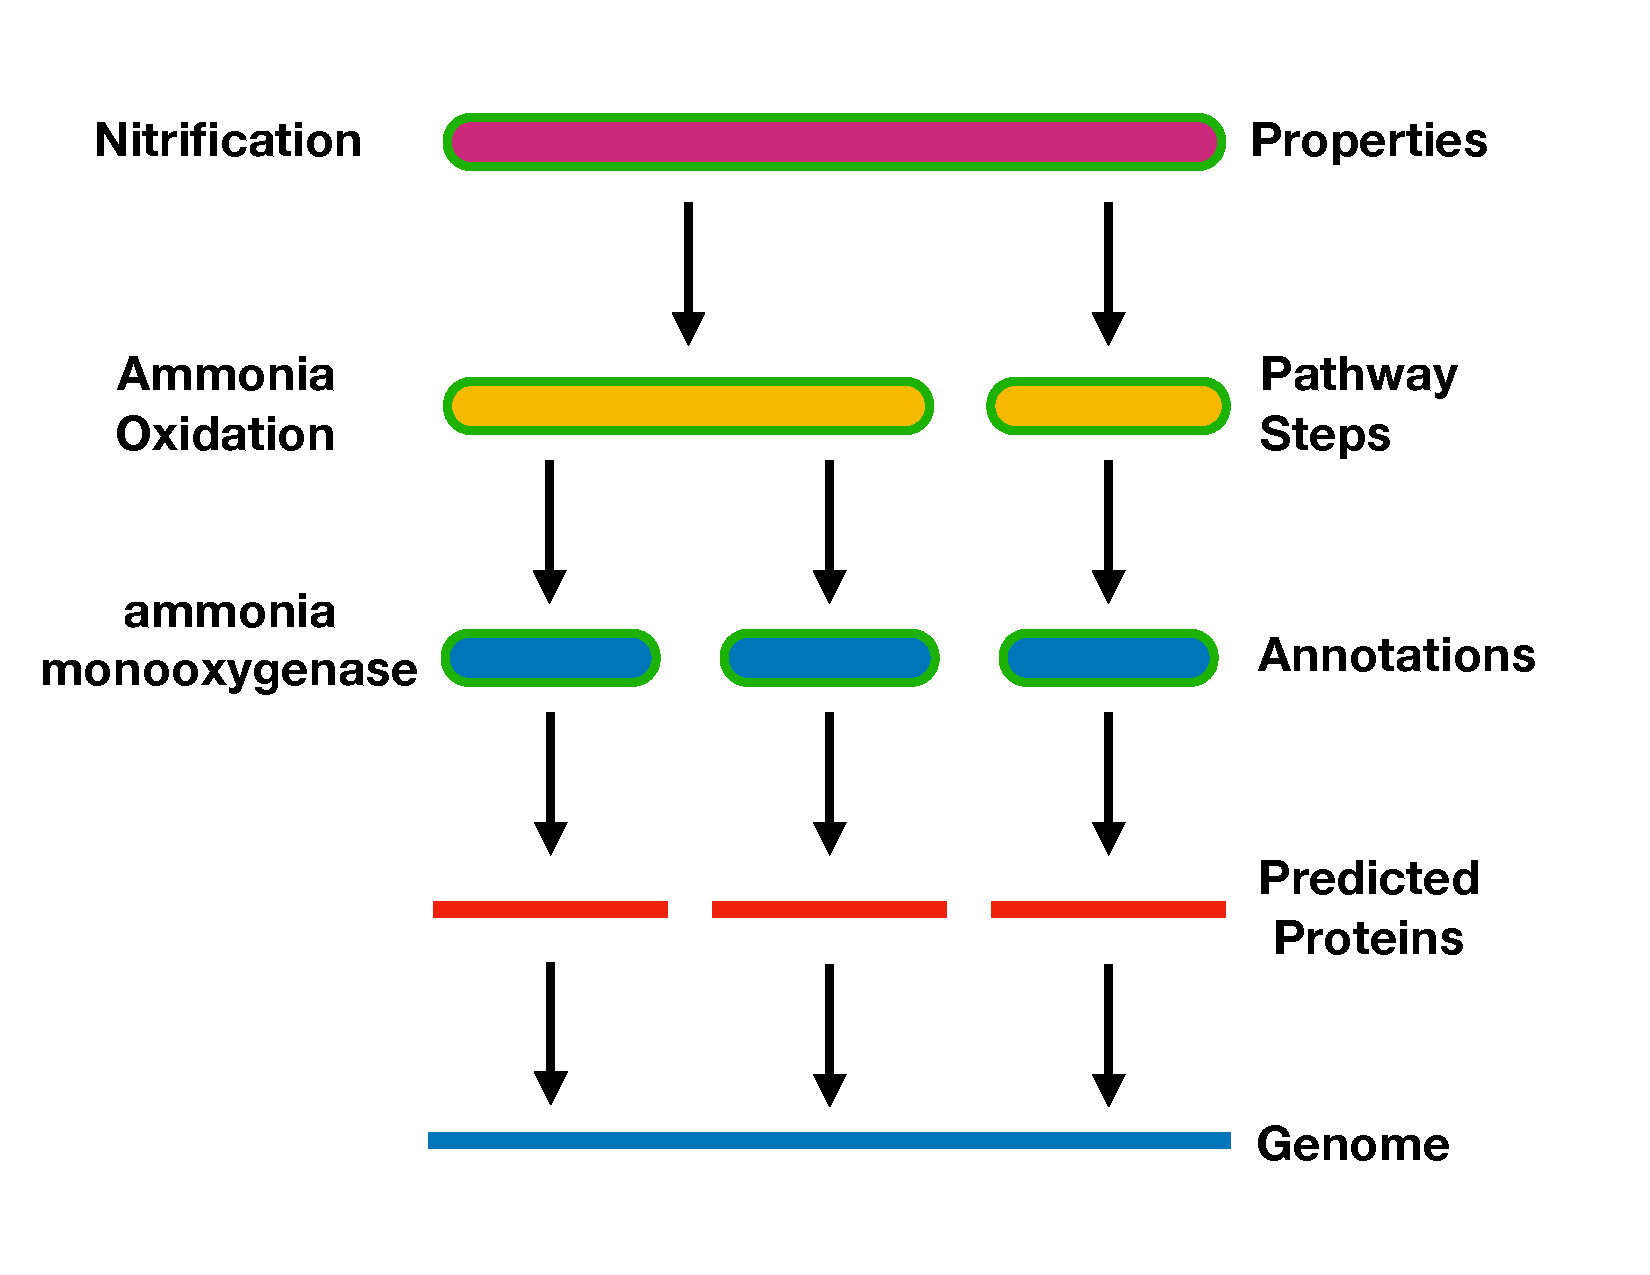
\includegraphics[width=0.9\textwidth]{media/pathway_analysis_steps.pdf}
	 \caption[The glyoxylate shunt is an example of a short biochemical pathway 
that can be genomically predicted.]{T\textbf{he glyoxylate shunt is an example 
of a short biochemical pathway that can be genomically predicted.} If a 
microorganism is to be classified as possessing this type of metabolism, then it 
should have highly similar proteins to those previously known to carry out the 
pathway. Several steps are required to go from an organism's genome sequence to 
a prediction of its metabolic capabilities. The enzymes that carry out pathway 
steps must be identified (\textit{e}.\textit{g}., protein annotation). If found, they indicate the 
presence of pathway steps. Finally, if all or many steps are present, then the 
biochemical pathway can be said to be present.}
	 \label{fig:pathway-analysis-steps}
\end{figure}

\begin{figure}[!ht]
  \centering
	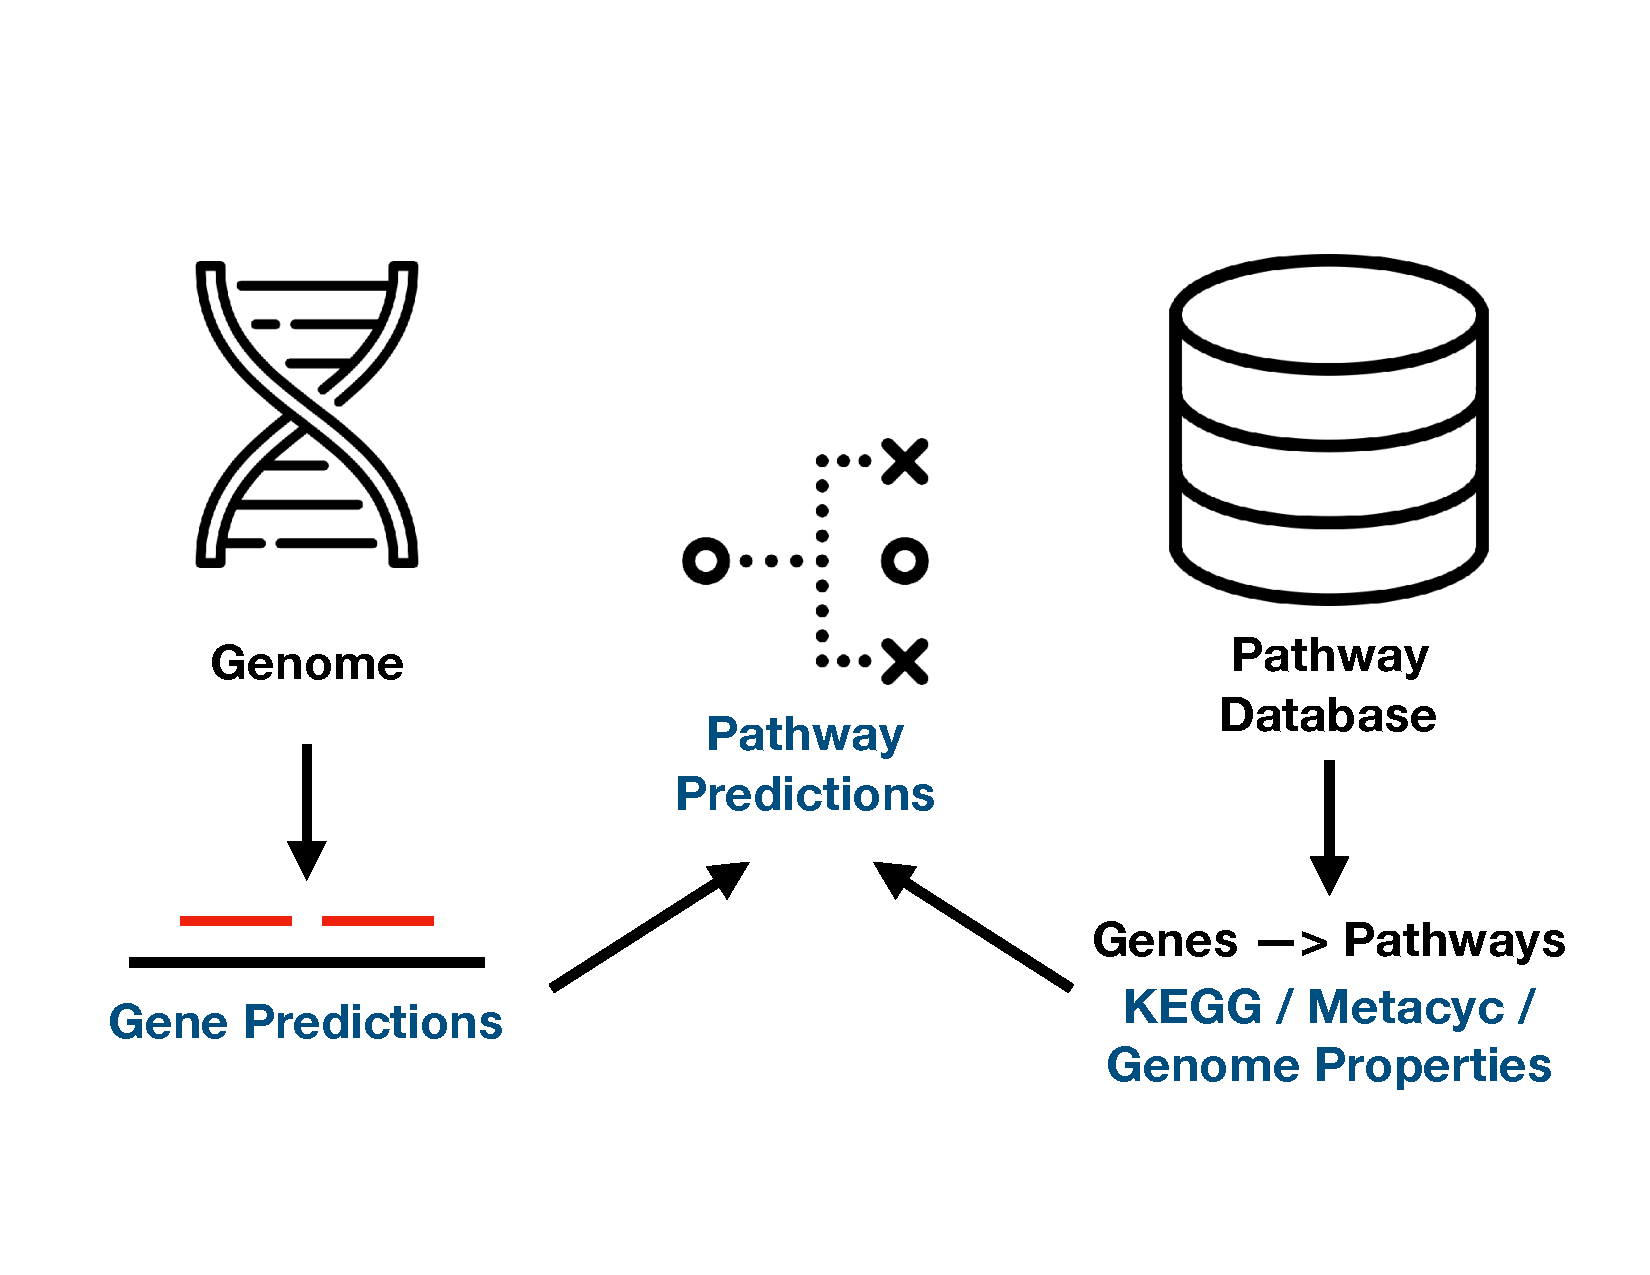
\includegraphics[width=0.8\textwidth]{media/pathway_bioinformatics.pdf}
	 \caption[Predicting an organism's biochemical pathways involves joining 
together two distinct data sets.]{\textbf{Predicting an organism's biochemical 
pathways involves joining together two distinct data sets.} One is a prediction 
of what genes are possessed by an organism. The other is a database containing 
the knowledge of what genes are involved in previously known biochemical 
pathways. When these previously cataloged genes are found within an organism's 
genome, pathway prediction can be made.}
	 \label{fig:pathway-analysis-overview}
\end{figure}

Users can deploy pathway prediction bioinformatics pipelines in two ways. They 
can either be installed on to a user's computer, where genomes can be processed 
directly, or be deployed on to a web server, where users can upload their 
genomes for remote processing. Some pipelines only work with pathway data from a 
specific database. For example, Pathway Tools \cite{karp2002pathway} can only 
present information about pathways found within the MetaCyc 
\cite{karp2002metacyc} database. Often pipelines are optimized for generating 
data from the genomes of a specific clade on the tree of life. For example, 
Prokka \cite{seemann2014prokka}, a pipeline that predicts genes and annotates 
protein sequences, is only designed to work with the genomes of prokaryotic 
microbes. Prokka only carries out the first few steps of the above list 
\cite{seemann2014prokka}. Once these proteins are predicted, they can be 
uploaded to servers such as \gls{kaas} \cite{moriya2007kaas} for pathway 
annotation. Some tools can perform all of the pathway analysis steps outlined in 
the list above. For example, \gls{rast} \cite{aziz2008rast} can take the upload 
of whole or partial bacterial genomes, predict the genes of these genomes, and 
provide users with a report displaying found pathways.

\section{The Current Bottlenecks of High Throughput Pathway Analysis}

Due to the current plethora of tools for genome annotation and pathway 
determination, identifying pathways for single organisms is becoming a solved 
problem. Researchers have progressed to comparing the presence and absence of 
pathways across organisms. Such comparisons are in the hope of finding 
information about individual organism's ecological roles, evolution, or 
suitability towards different industrial tasks. For example, the genomes of 
organisms that are closely related phylogenetically could be compared to 
determine those that may have lost or gained a pathway or pathway step over time 
(Fig. \ref{fig:phylogenetic-comparison}). Alternatively, the pathways possessed 
by multiple organisms from within the same environment could be compared to shed 
light on their potential ecological niches (Fig. \ref{fig:metagenomics}). 
Pathway comparisons could also be used industrially to select organisms to add 
to bioprocess co-cultures.

\begin{figure}[!ht]
  \centering
	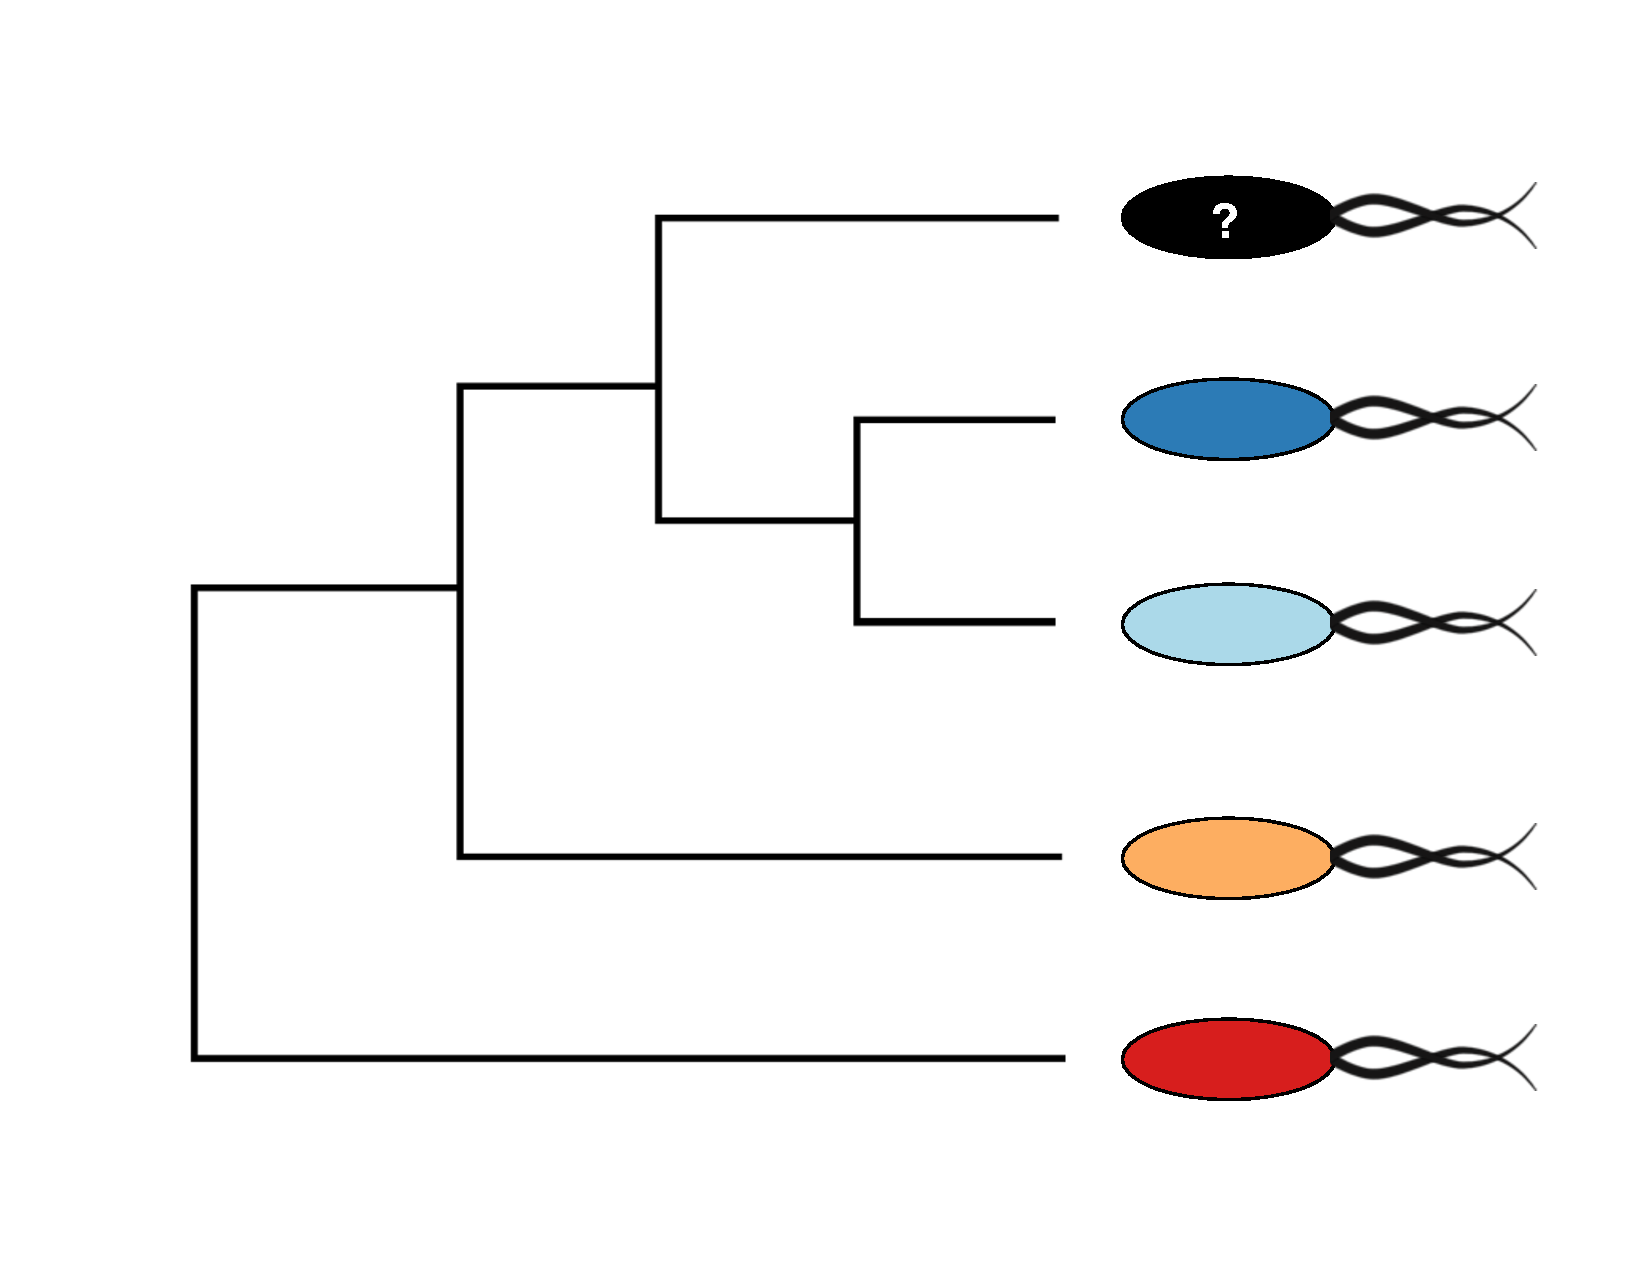
\includegraphics[width=0.7\textwidth]{media/compare-phylogenetically.pdf}
	 \caption[When a new microorganism is discovered it is useful to compare its 
metabolism to those of closely related taxa.]{\textbf{When a new microorganism 
is discovered it is useful to compare its metabolism to those of closely related 
taxa.} A novel organism (black) placed within a phylogenetic tree, represented 
here by a dendrogram, to identify its sister taxa. Both pathway prediction and 
phylogeny can be predicted from an organism's genome.}
	 \label{fig:phylogenetic-comparison}
\end{figure}

\begin{figure}[!ht]
  \centering
	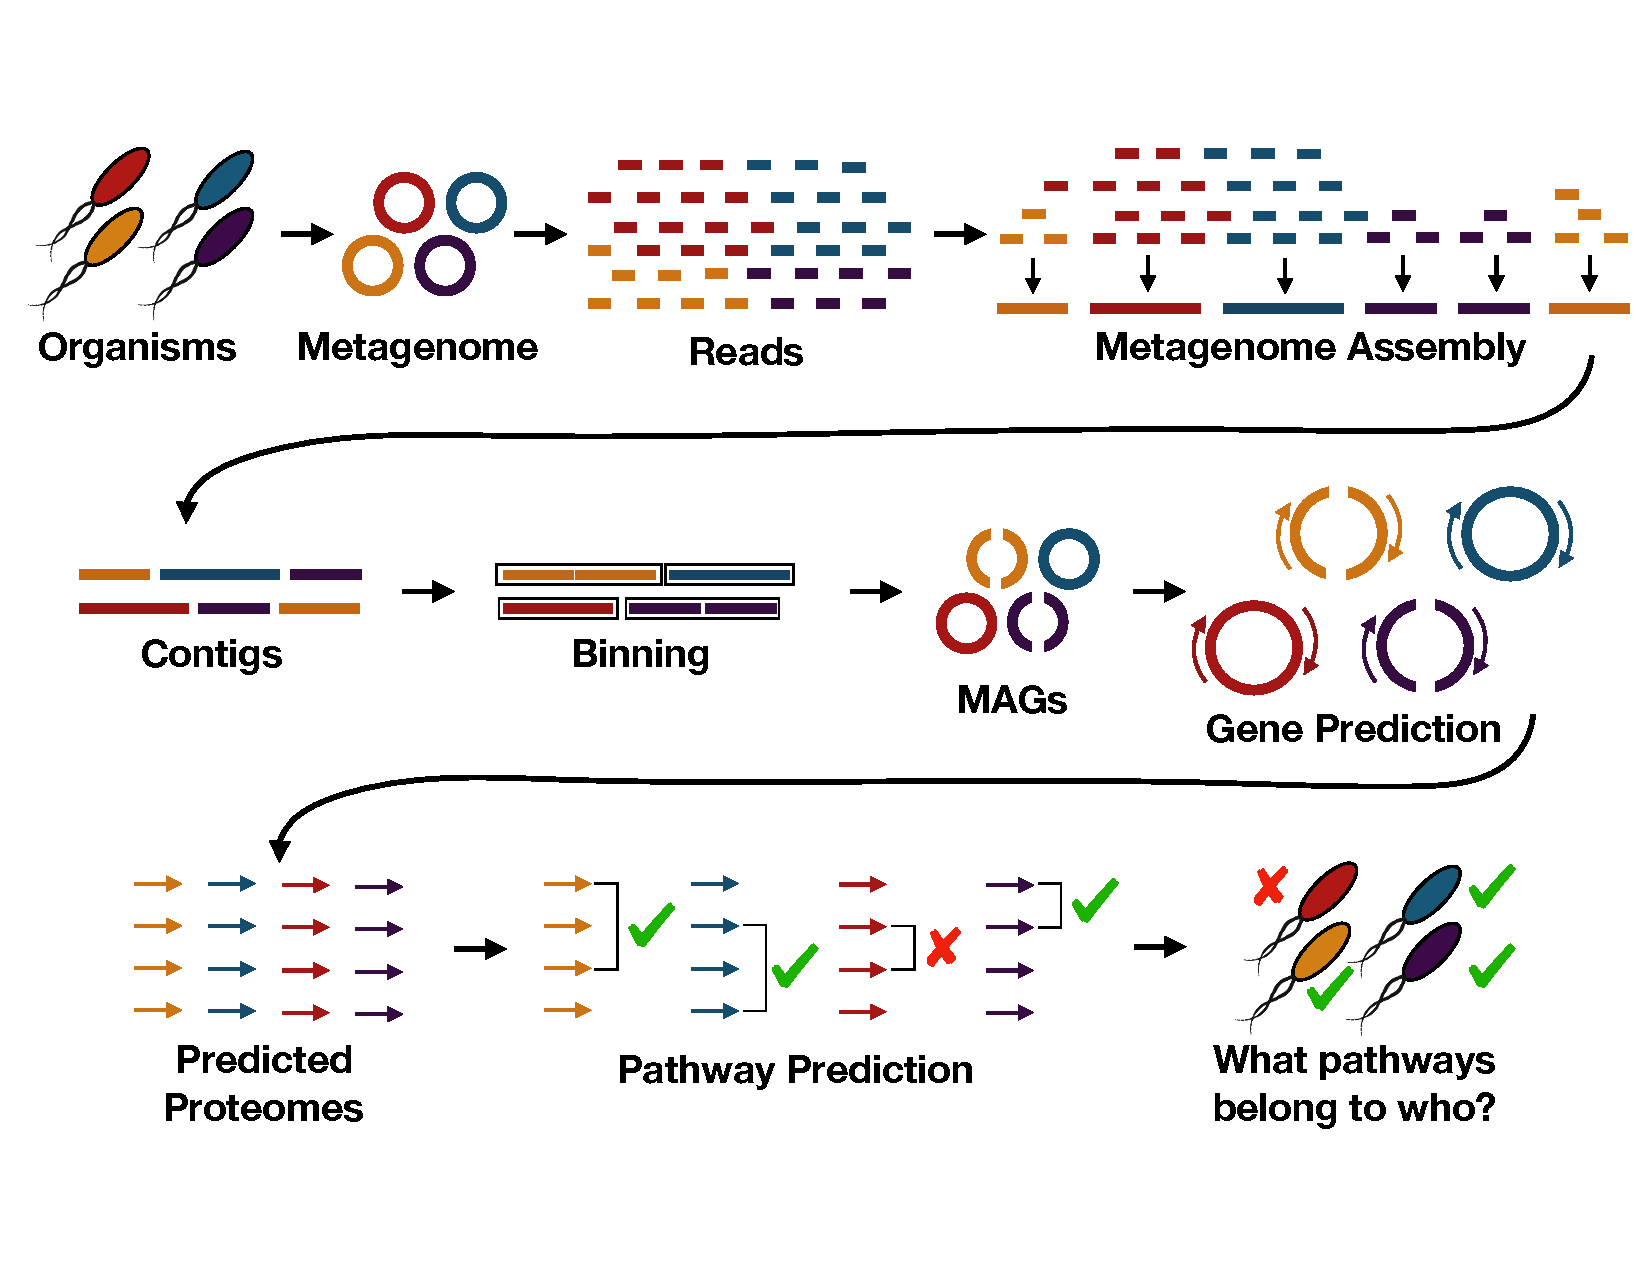
\includegraphics[width=0.75\textwidth]{media/metagenomics.pdf}
	 \caption[Metagenomics can be used to compare the predicted pathways of 
multiple organisms found within the same environmental 
sample.]{\textbf{Metagenomics can be used to compare the predicted pathways of 
multiple organisms found within the same environmental sample.} Bioinformatics 
techniques can be used to separate individual genomes from a metagenomic sample. 
Pathway annotation can be performed on these genomes and used to compare the 
pathways possessed by different organisms from the same environment. Such 
comparisons can be used to evaluate each organism's potential role in an 
environment.}
	 \label{fig:metagenomics}
\end{figure}

Although assigning pathway presence and absence to individual organisms can be 
done quite rapidly, the comparison of these results across multiple organisms is 
currently a considerable bottleneck in the area of pathway analysis. Often 
pathway annotation tools that can process multiple genomes simultaneously 
present their results in the form of computer spreadsheets (\textit{e}.\textit{g}., Microsoft 
Excel or \gls{csv} files \cite{RFC4180}). After generation of these 
spreadsheets, users are required to manually scan through the thousands of 
pathway rows and organism columns to find pathway differences across organisms. 
Researchers with data science and coding skills may be able to generate custom R 
or Python scripts that assist them in this task by filtering down these 
spreadsheets to show only pathways that are different or by generating data 
visualizations that accelerate pattern detection. To accelerate script 
development, libraries have been written to help scriptwriters interact with 
pathway data. However, the majority of these libraries focus on helping users 
download data from existing pathway databases, rather than helping them with 
making comparisons across organisms. Thus, due to a lack of libraries for 
pathway comparison and lack of coding skills among biologists, there is a need 
for dedicated bioinformatics tools that simply pathway comparisons across 
organisms. Software that visualizes the presence and absence of pathways these 
would be of great use in this role. There are several emerging tools, which are 
discussed in Section \ref{micromeda-client-summary}, that help users visualize 
pathway annotations from multiple organisms. However, their implementation, in 
terms of visual idioms used and supporting data presented, is currently lacking. 
There is currently a gap for a tool that effectively presents such data and 
allows for rapid comparisons. There is also a gap for a pathway library that 
assists coders in making these comparisons programmatically. Finally, there is a 
gap for a tool that can both users what pathways an organism possess and allows 
users to identify the protein sequences that support these annotations. 
Micromeda and Pygenprop were developed to fill these gaps.

\section{The Micromeda Platform} \label{micromeda-overview}

The bioinformatics system presented within this thesis, called Micromeda, is 
designed to address current gaps in the researcher's ability to compare pathway 
presence and absence across organisms. The platform does this without losing 
information about the protein sequences that support these pathways' existence. 
The output of the platform is an interactive heat map that displays rows of 
pathways by columns of organisms (Fig. \ref{fig:basic-heatmap-overview}). Heat 
map cells are coloured by the level of support for a pathway's existence in each 
genome (Fig. \ref{fig:basic-heatmap-overview}). This data visualization is 
displayed within a user's web browser. As discussed in Chapter 
\ref{micromeda-client}, this heat map is interactive, and users can tailor it to 
only display presence and absence for specific pathways or pathway steps. A 
software stack (see 
\href{http://en.wikipedia.org/wiki/Solution_stack}{en.wikipedia.org/wiki/Solution\_stack}) 
consisting of several components, some of which were developed as part of the 
thesis project, is used to generate data for the visualizations that Micromeda 
presents. This stack is outlined in the list below.

\begin{figure}[!ht]
  \centering
	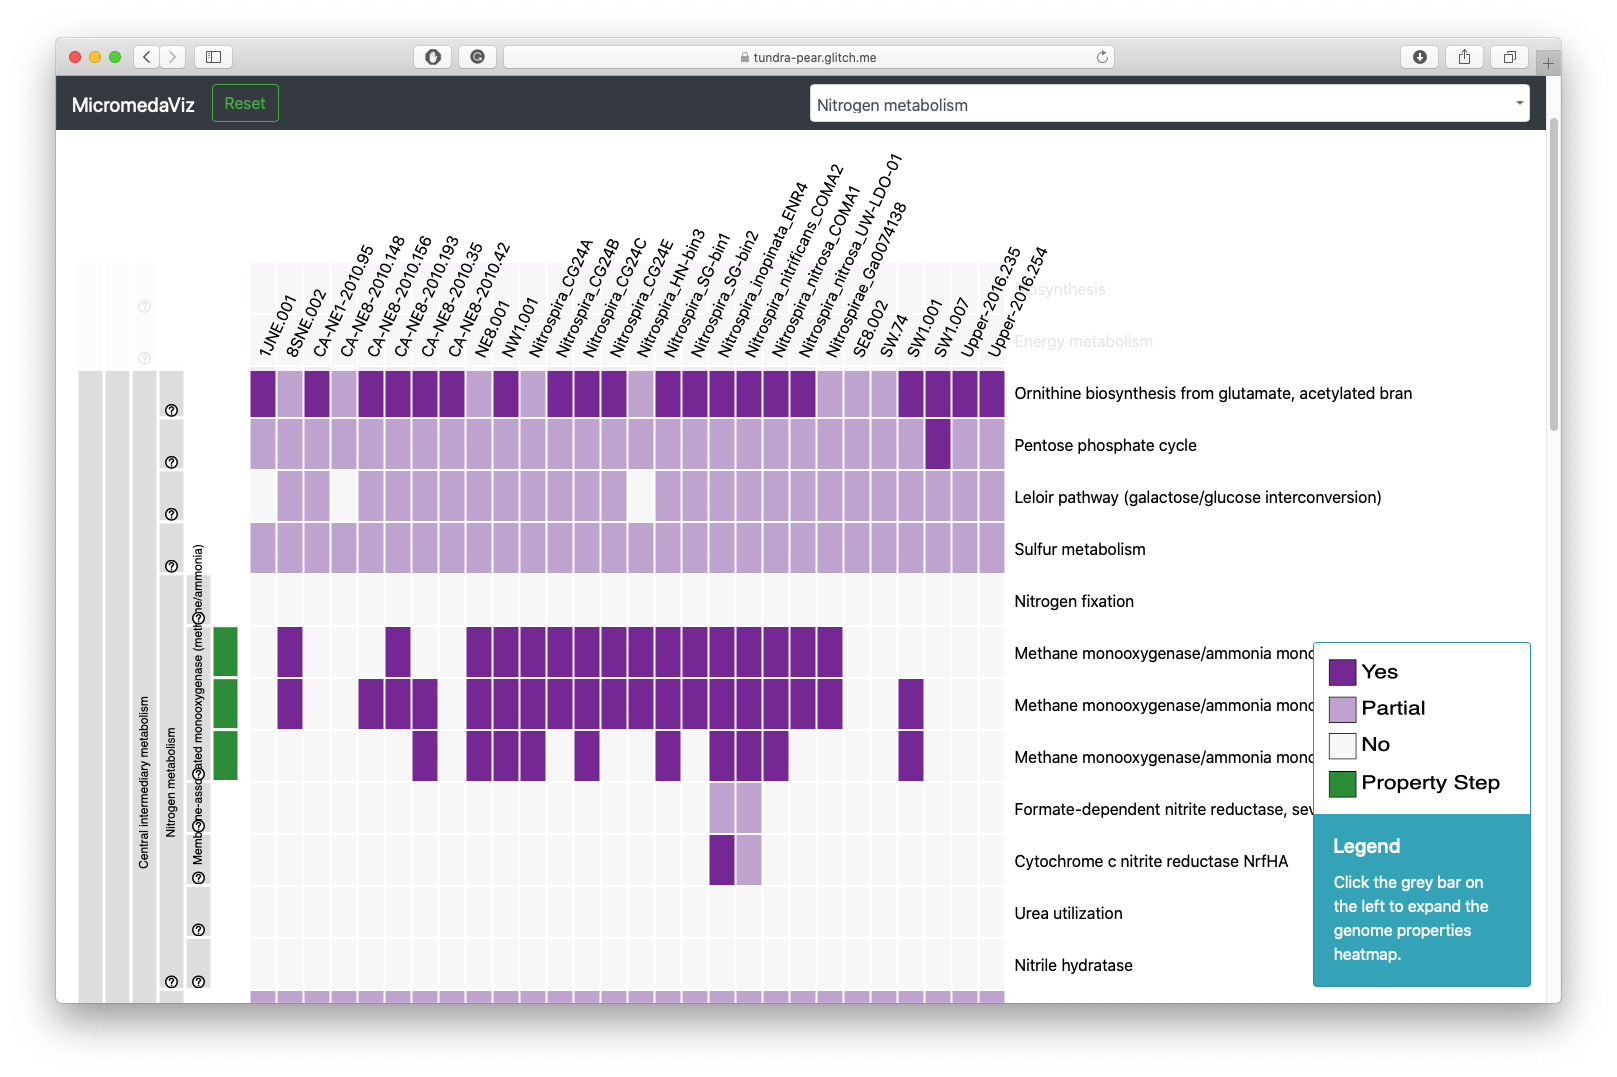
\includegraphics[width=0.9\textwidth]{media/Micromeda-Simple-Overview.png}
	 \caption[Micromeda's user interface generates a pathway heat map 
visualization.]{\textbf{Micromeda's user interface generates a pathway heat map 
visualization.} This heat map consists of pathway rows by organism columns and 
allows the comparison of pathway presence and absence across organisms. All 
other components of Micromeda were built to support this interface by providing 
it with data. Further explanation of the interface's design can be found in 
Chapter \ref{micromeda-client}.}
	 \label{fig:basic-heatmap-overview}
\end{figure}

\begin{itemize}
\item A client web application that runs in the user's browser. This web 
application allows users to upload files to a server. These files contain 
precalculated data about an organism's predicted pathways and the protein 
sequences that support these predictions. This application draws the pathway 
heat maps mentioned above based on the data uploaded (Fig. 
\ref{fig:basic-heatmap-overview}). These heat maps allow users to make 
comparisons across pathways and organisms. This component is called 
\textbf{Micromeda-Client} and is detailed in Chapter \ref{micromeda-client}. 
Links to a demonstration of the client interface can be found in Section 
\ref{client-demo}.
\item A server web application that runs on a remote computer system and in 
support of the client application. This server application accepts the above 
file upload and provides the client with easy access to the data held within the 
file. This component is called \textbf{Micromeda-Server} and is discussed in 
Chapter \ref{micromeda-server}.
\item A file format that allows users to easily transfer an assessment of what 
pathways are possessed by multiple organisms and the protein sequences used to 
support this assessment. These files, called \textbf{Micromeda files}, are the 
files uploaded to Micromeda-Server and use a custom format that is discussed in 
Section \ref{MicromedaFiles}. The format allows for the storage of the above 
information in the most compact way possible.
\item A software library that supports the generation of pathway annotations, 
rapid programmatic comparisons between organism pathway annotations and the 
generation of the above Micromeda files. The library is compatible with many 
emerging machine learning tools and opens up new avenues to their application to 
pathway analysis. This library is called \textbf{Pygenprop} and is discussed in 
Chapter \ref{Pygenprop}.
\item A pathway database that maps between predicted protein sequences derived 
from an organism's genome and biochemical pathway steps. The database chosen was 
the \textbf{Genome Properties} database \cite{richardson2018genome}. A short 
review of this database and the reason for its selection can be found in Chapter 
\ref{genome-properties}. This database is pre-existing and was not made as part 
of the thesis work.
\item A pre-existing sequence search program for scanning for identifying 
markers within the sequences of an organism's predicted proteins. These markers 
are used to identify enzymes that support the existence of a pathway. The search 
program chosen was \textbf{InterProScan5}, whose output data is used by the 
Genome Properties Database. An overview of InterProScan5 
\cite{jones2014interproscan} and its methodology can be found in Chapter 
\ref{genome-properties}.
\item A program that generates protein sequences from predicted genes found 
within an organism's genome. For example, in the case of prokaryotic genomes, an 
existing tool such as \textbf{Prodigal} \cite{hyatt2010prodigal} would be used. 
\end{itemize}

\begin{figure}[!ht]
  \centering
	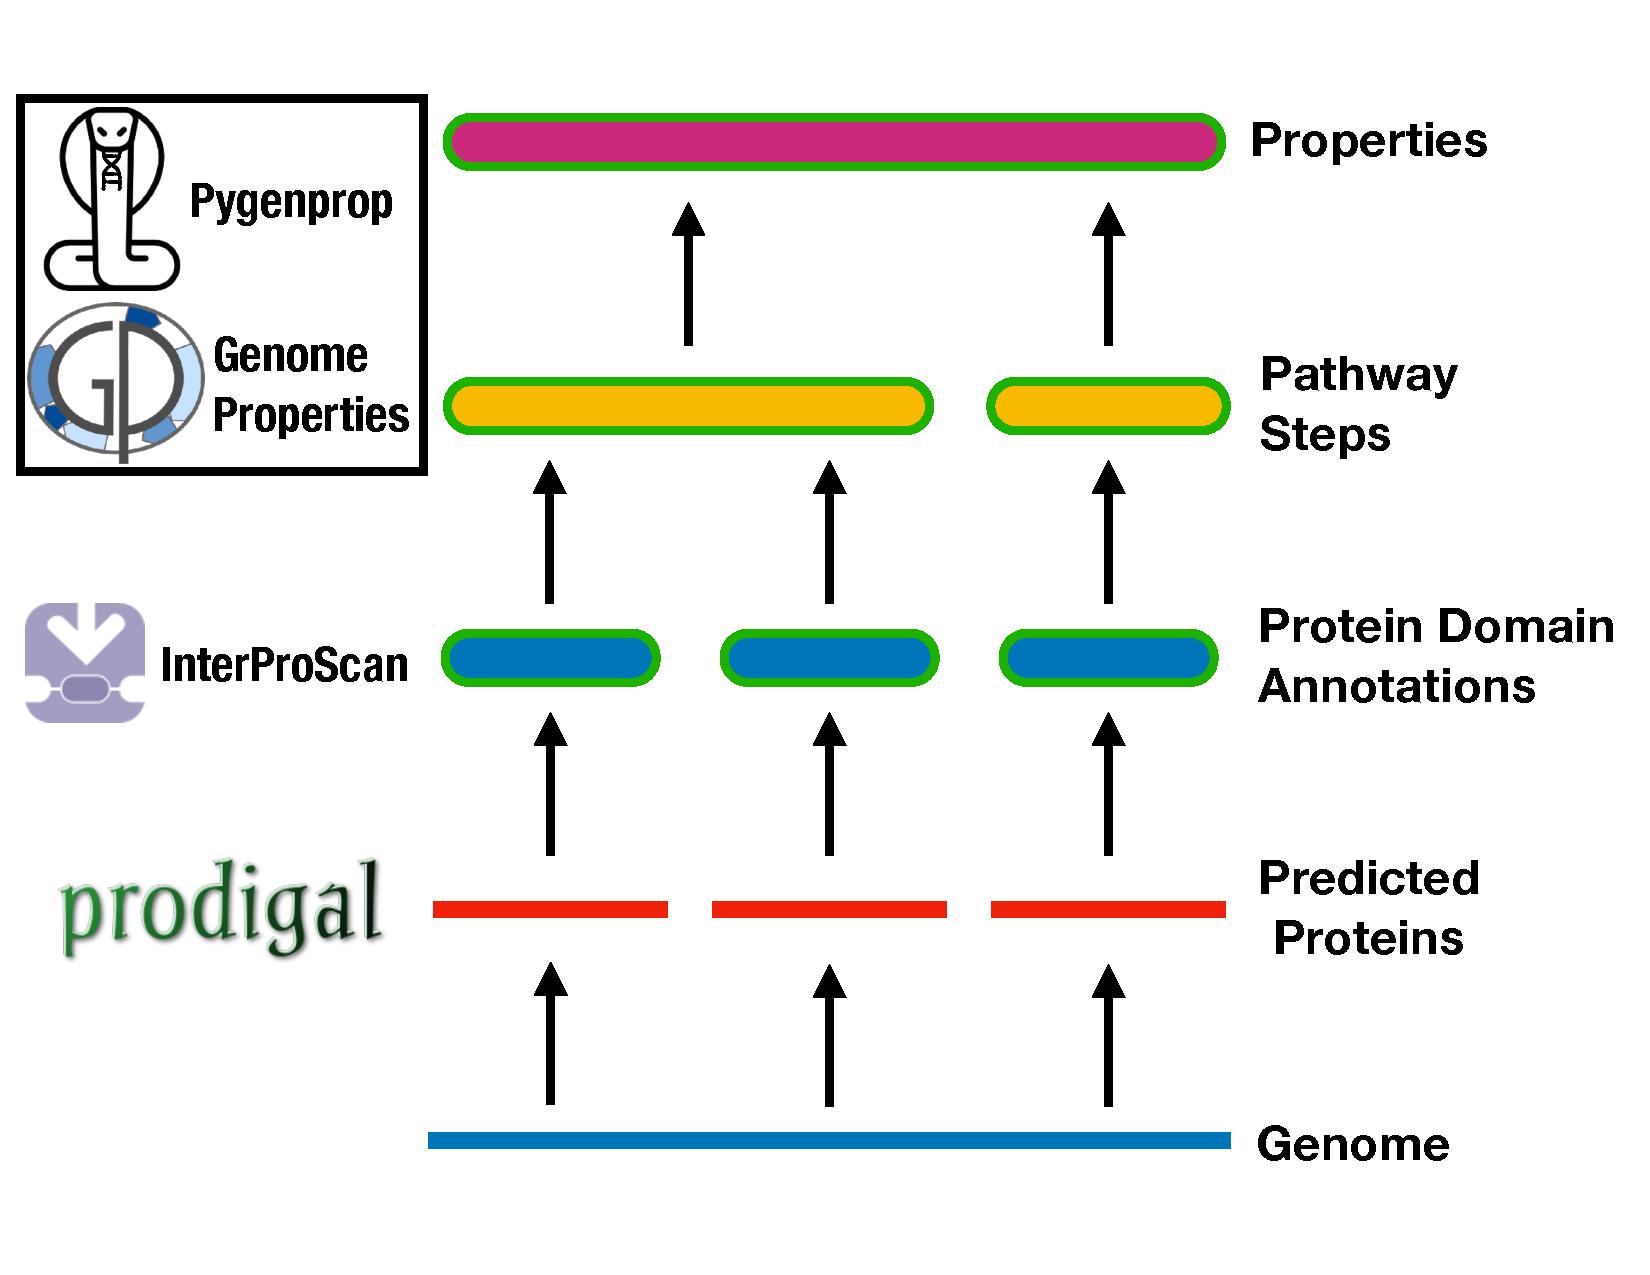
\includegraphics[width=0.8\textwidth]{media/micromeda-pipeline.pdf}
	 \caption[Micromeda carries out several steps that allow it to map from an 
organism's genome to predictions of what pathways are possessed by the 
organism.]{\textbf{Micromeda carries out several steps that allow it to map from 
an organism's genome to predictions of what pathways are possessed by the 
organism.} For prokaryotes,  proteins must firsts be predicted via Prodigal. 
These proteins are then scanned using InterProScan5. The results of InterProScan 
are then combined with the Genome Properties database to predict pathways steps. 
These predictions are carried out by Pygenprop, which also predicts the overall 
presence and absence of pathways.}
	 \label{fig:micromeda-levels}
\end{figure}

\begin{figure}[!ht]
  \centering
	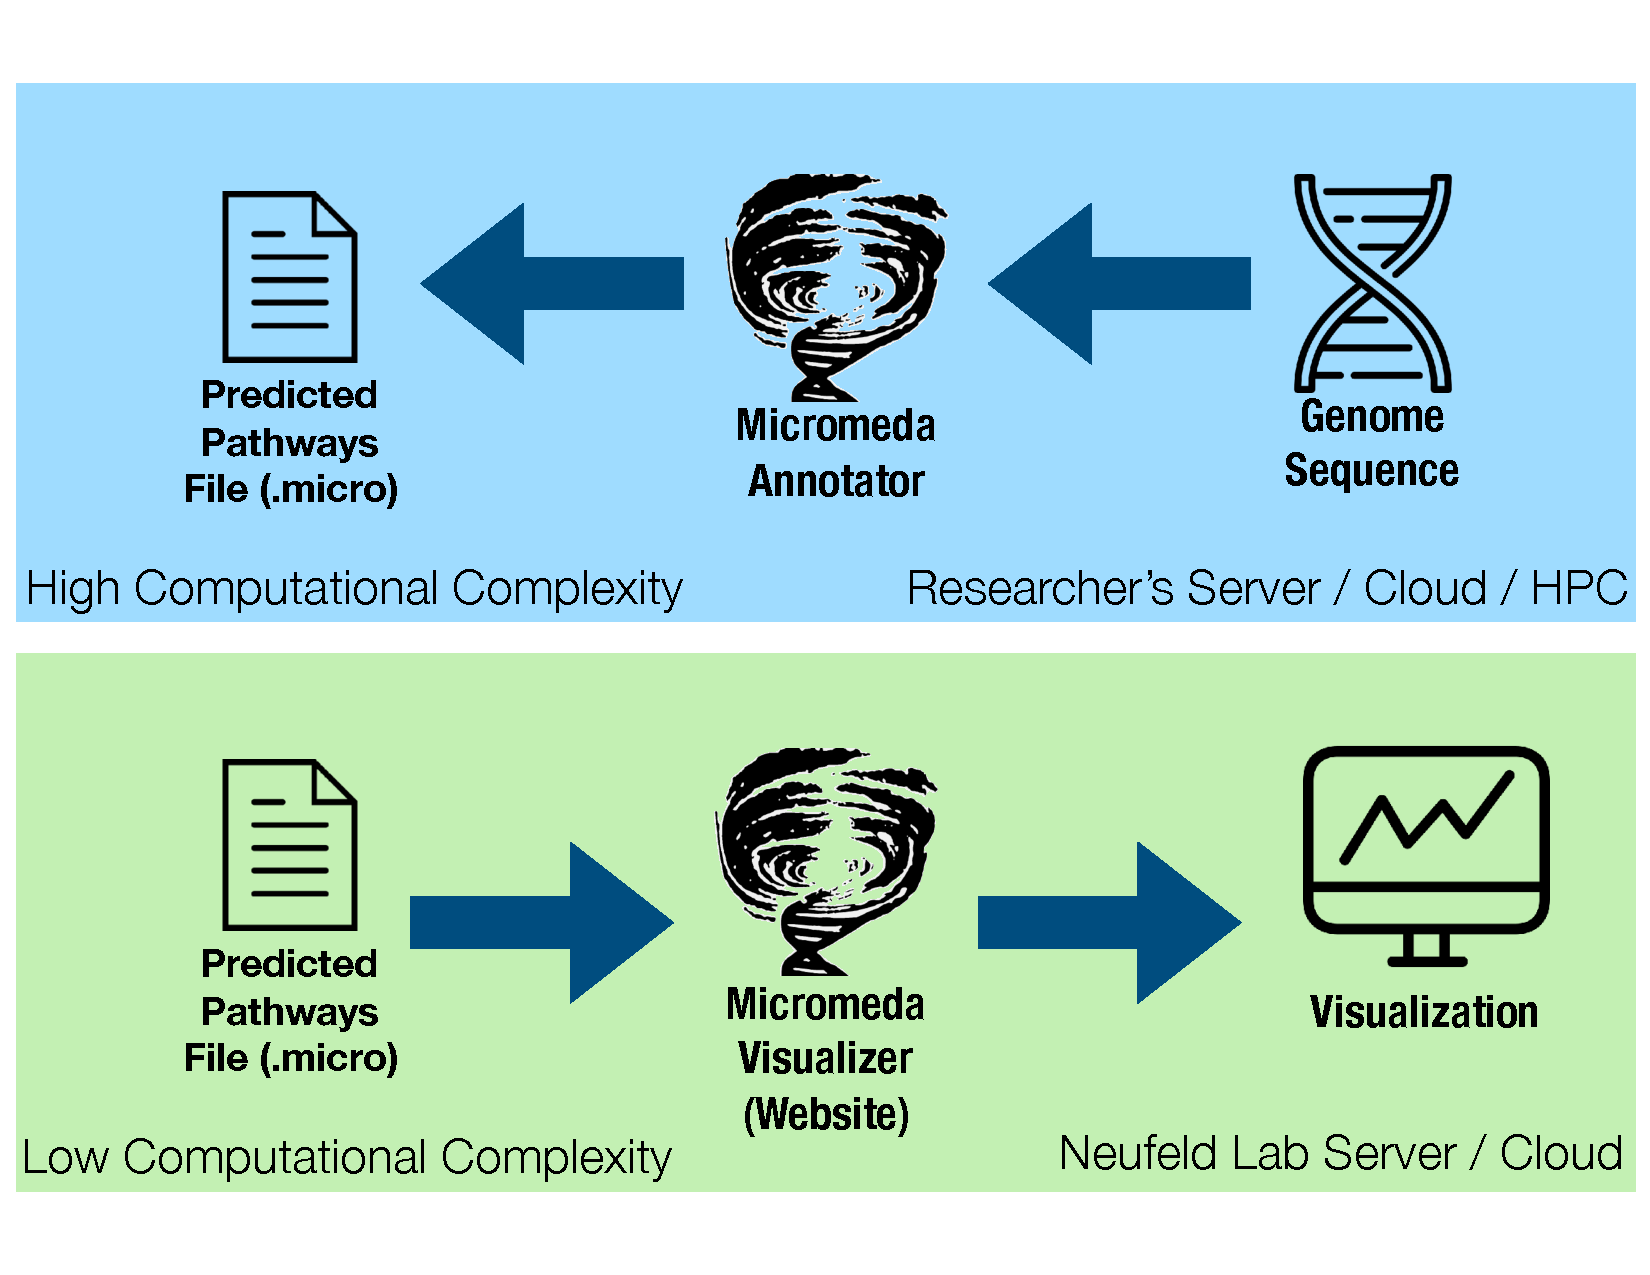
\includegraphics[width=0.8\textwidth]{media/micromeda-file-generation.pdf}
	 \caption[With Micromeda, the computation that generates pathway visualizations 
is split across two different computer systems.]{\textbf{With Micromeda, the 
computation that generates pathway visualizations is split across two different 
computer systems.} One local computer system executes a data generation step 
that creates a Micromeda file. Users then uploaded this file to a second remote 
computer system that helps generate heat map visualizations. The most 
computationally complex step, Micromeda file generation, is not performed on the 
same server that generates the data visualizations.}
	 \label{fig:micromeda-file-generation}
\end{figure}

\begin{figure}[!ht]
  \centering
	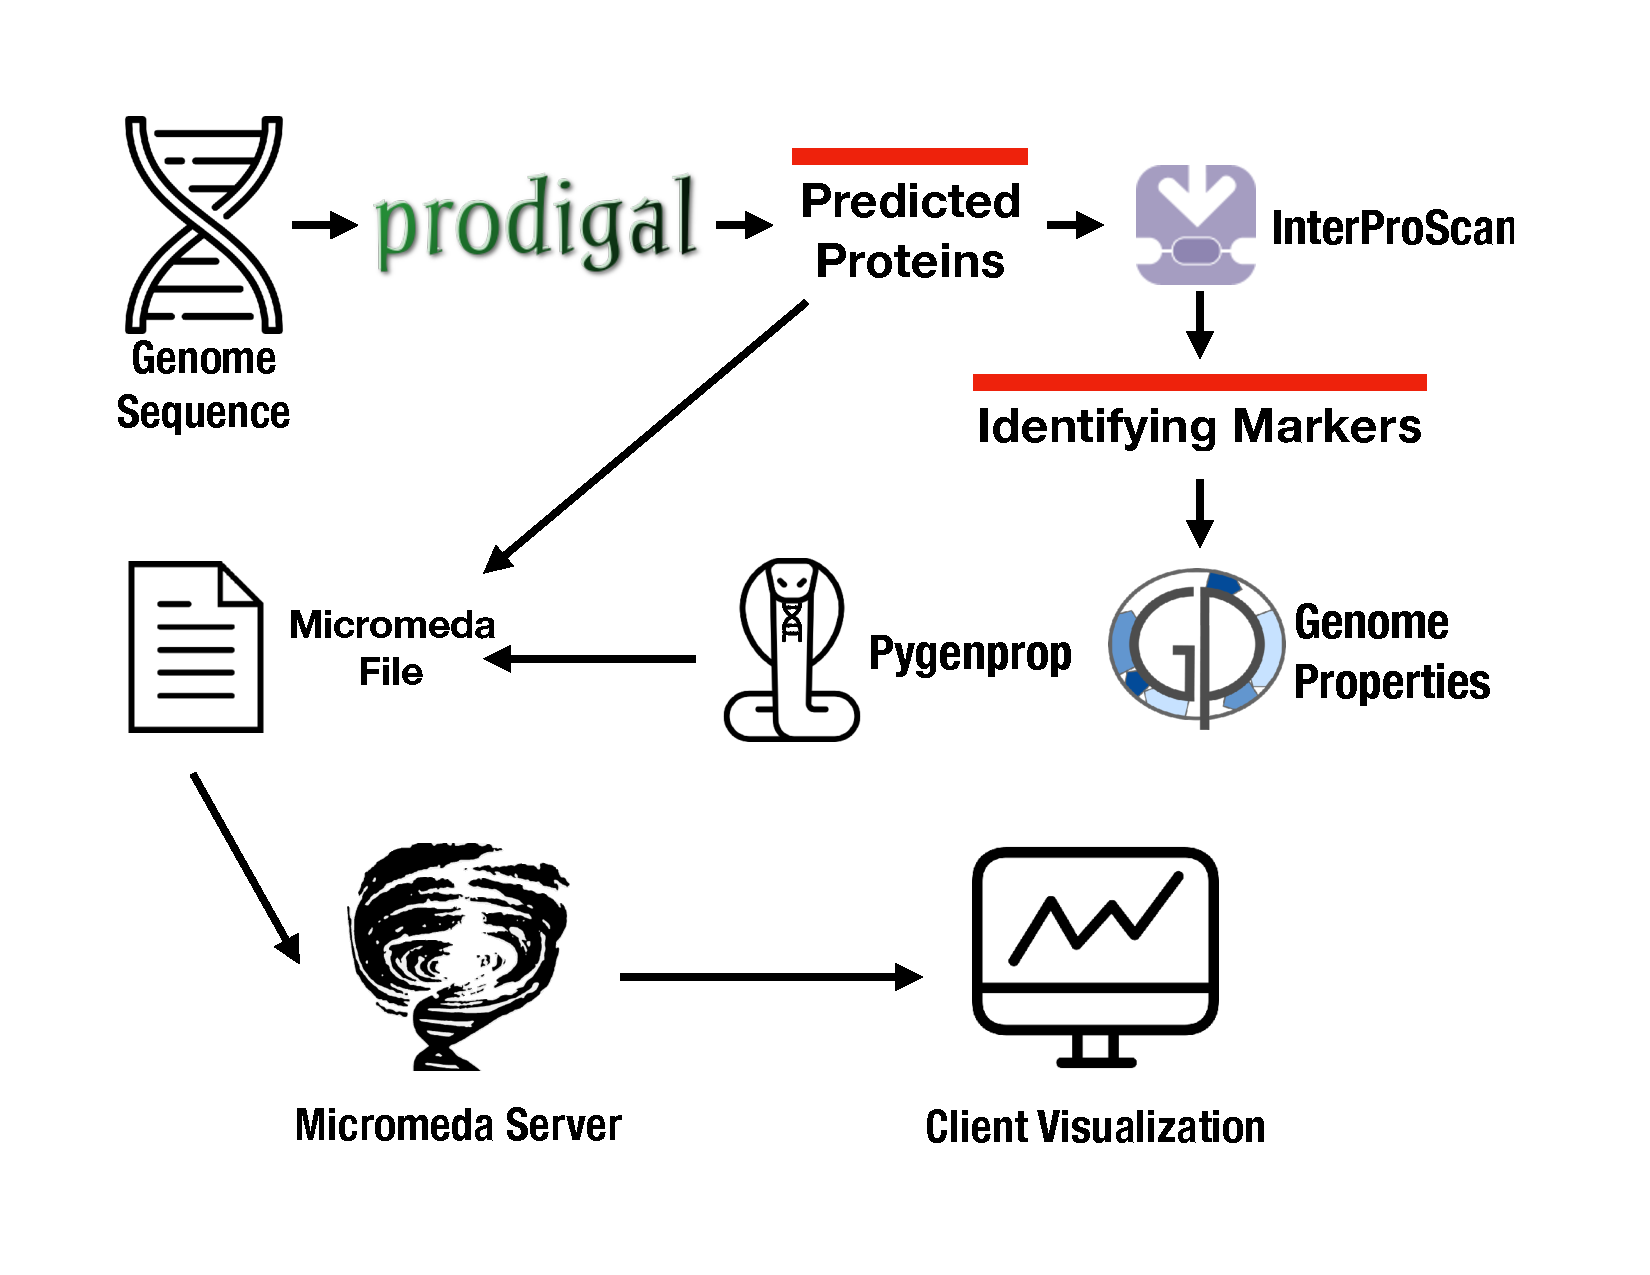
\includegraphics[width=0.8\textwidth]{media/how-micromeda-files-are-built.pdf}
	 \caption[Micromeda files are built from InterProScan annotations of an 
organism's predicted proteins.]{\textbf{Micromeda files are built from 
InterProScan annotations of an organism's predicted proteins.} They possess not 
only pathway annotations but also the protein sequences that support them. Thus 
they allow for the transfer complete pathway datasets. Micromeda files are 
uploaded to a remote server for visualization.}
	 \label{fig:micromeda-file-building-and-use}
\end{figure}

The above Micromeda platform can be subdivided into two core components: a 
toolchain for generating Micromeda files (labelled Micromeda Annotator in Fig. 
\ref{fig:micromeda-file-generation}) and a web application for visualizing the 
data they contain (labelled Micromeda Visualizer in Fig. 
\ref{fig:micromeda-file-generation}). The individual steps for generating 
Micromeda files can be done manually using only three \gls{cli} tools (see Fig. 
\ref{fig:micromeda-levels}, Fig. \ref{fig:micromeda-file-building-and-use}, and  
\href{http://en.wikipedia.org/wiki/Command-line_interface}{en.wikipedia.org/wiki/Command-line\_interface}). 
For example, with prokaryotic genomes, Prodigal could be used to predict protein 
sequences from an organism's genome sequence, and InterProScan5 could be used to 
scan these proteins to identify enzymes that support the existence of specific 
pathways (Fig. \ref{fig:micromeda-file-building-and-use}). Afterwards, a Python 
script taking advantage of the Pygenprop library could be used to convert the 
output from InterProScan and Prodigal a Micromeda file. This script would also 
use a copy of the Genome Properties database (Fig. 
\ref{fig:micromeda-file-building-and-use}). An example of such a script can be 
found within Pygenprop's GitHub repository 
(\href{http://github.com/Micromeda/pygenprop}{github.com/Micromeda/pygenprop}). 
An explicit automated software pipeline for generating Micromeda files does not 
currently exist. However, its potential implementation is discussed in 
Subsection \ref{pipeline-development}.

\subsection{Software Architecture Overview}

Micromeda follows a client-server web architecture \cite{svobodova1985client} 
(see 
\href{http://en.wikipedia.org/wiki/Client-server_model}{en.wikipedia.org/wiki/Client-server\_model} 
and Section \ref{web-servers}). Users interact with Micromeda-Client via their 
web browser, and it allows them to upload Micromeda files to Micromeda-Server. 
Micromeda files contain all the information that the client requires to generate 
a pathway heat map. These files store pathway annotations, InterProScan5 output 
data, and supporting protein sequences for multiple organisms (see Section 
\ref{MicromedaFiles}). Having all these datasets in a single file simplifies the 
data upload process as only one file has to be uploaded by the user per heat map 
drawn. After upload, the contents of the uploaded file are stored temporarily in 
\gls{ram} on the computer used to host Micromeda-Server (see Section 
\ref{server-workflow}). Micromeda-Client will ask Micromeda-Server for data from 
this file as it draws a heat map or responds to user activity (see Section 
\ref{client-implementation}). Multiple users can interact with Micromeda-Server 
and Client simultaneously.

\subsection{The Reasoning for Building a Web Application and Having Micromeda 
files} \label{why-micromeda-files}

Micromeda's \gls{ui} runs inside a user's web browser. The reasoning for using 
this approach, in contrast to building Micromeda as a native desktop 
application, is discussed in Section \ref{client-delivery-method}. The reason 
Micromeda files exist is that they allow the rapid transfer of pathway 
annotation datasets that, in turn, allow for a separation of data generation and 
visualization. This separation is essential because there are vast computational 
complexity differences between creating pathway annotations and visualizing 
their contents. Micromeda's pathway prediction method involves identifying 
specific enzymes by running InterProScan5 on the set of all predicted proteins 
of an organism. The algorithms used by InterProScan5 are very computationally 
complex. It takes on the order of two hours to scan through the 4313 proteins of 
\textit{E. coli} K12 (\gls{ncbitaxa}: 1010810) using 100\% of all the \gls{cpu} 
cores of a 16 core server\footnote{InterProScan5 was tested on a server with two 
Intel E5310 (4 \gls{cpu} cores/4 threads/8 \gls{mb} cache/1.60 \gls{ghz} clock 
speed) processors and 16 \gls{gb}  of \gls{ram}.}.

In contrast, Micromeda can render a pathway heat map for over forty organisms in 
less than a second. Thus, if one wanted to have a web application that both 
computes and visualizes pathway annotations for uploaded genome sequences, it 
would require the support of an extensive and well-maintained hardware 
infrastructure. Developing the code to build, maintain, and sustain such a 
system draws away from the core goal of the Micromeda platform, which was to 
design a tool that helps users visualize pathway differences across organisms. 
Hence, for Micromeda, I chose to have users generate pathway annotations 
locally, using InterProScan5 and other tools, and have them upload these files 
to a remote web server for visualization (Fig. 
\ref{fig:micromeda-file-generation}). This design decision significantly reduces 
the hardware requirements for those who want to host Micromeda-Server and 
Client. It also reduces the overall design complexity of Micromeda-Client and 
Server and allows future development to focus on creating better and more 
feature-rich versions of Micromeda's \gls{ui} and visualizations.

\section{Summary} \label{introduction_summary}

Micromeda allows users to visualize the differences in pathway presence and 
absence across organisms. It does this based on the data contained within 
uploaded Micromeda files. Pygenprop is a software library that can not only 
produce Micromeda files but also make programmatic comparisons of pathway 
presence and absence across organisms. Potential improvements to individual 
components of Micromeda are highlighted in the summary section of each of their 
chapters. Potential improvements that would require modification of multiple 
components are highlighted in Chapter \ref{conclusion-chapter}. As discussed in 
Chapter \ref{conclusion-chapter}, Micromeda breaks new ground in both features 
and implementation and will increase both the speed and ease at which 
researchers perform pathway analysis.
